\section{\texorpdfstring{Control Web - Aplikace}{Control Web - Aplikace}}

% =====================================================================================================================
	\begin{frame}
    \frametitle{Zadání}
		
		\begin{enumerate}
			\item Plnit a vyprazdňovat zásobník přítokem a odtokem,
			\item spínat okamžik plnění nebo vyprazdňování,
			\item ovládat rychlost plnění a vyprazdňování,
			\item hlídat dosažení maxima a minima hladiny zásobníku:
			
			\begin{itemize}
				\item podtékání,
				\item přetékání,
			\end{itemize}
			
		\end{enumerate}
		
		\vspace{3mm}
		Prakticky jde o zadání samostatné úlohy na cvičení.
	\end{frame}
	
% =====================================================================================================================
	\begin{frame}
    \frametitle{Aplikace - návrh}
		
		\begin{center}
			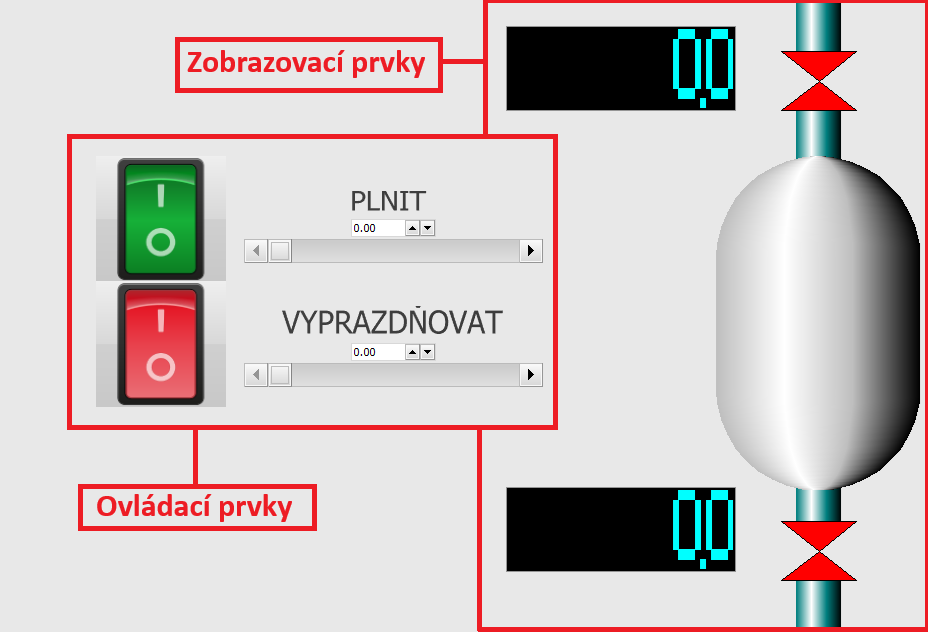
\includegraphics[width=0.85\textwidth]{fig/program_ukol_a.png}
		\end{center}
		
	\end{frame}
	
% =====================================================================================================================
	\begin{frame}
    \frametitle{Aplikace - řízení}
		
		\begin{center}
			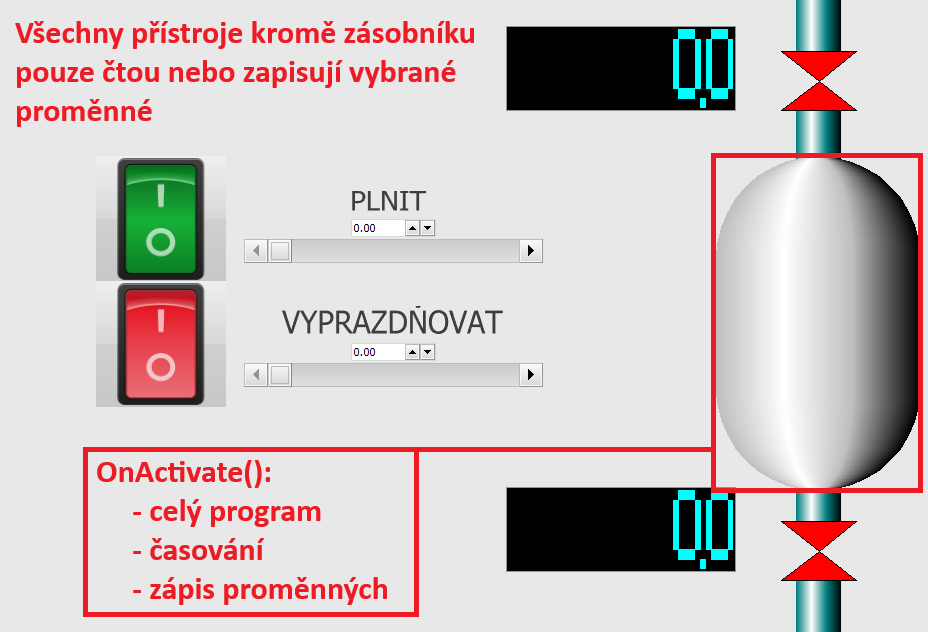
\includegraphics[width=0.85\textwidth]{fig/program_ukol_b.png}
		\end{center}
		
	\end{frame}
	
% =====================================================================================================================
	\begin{frame}
    \frametitle{Aplikace - podmínky}
		
		\begin{center}
			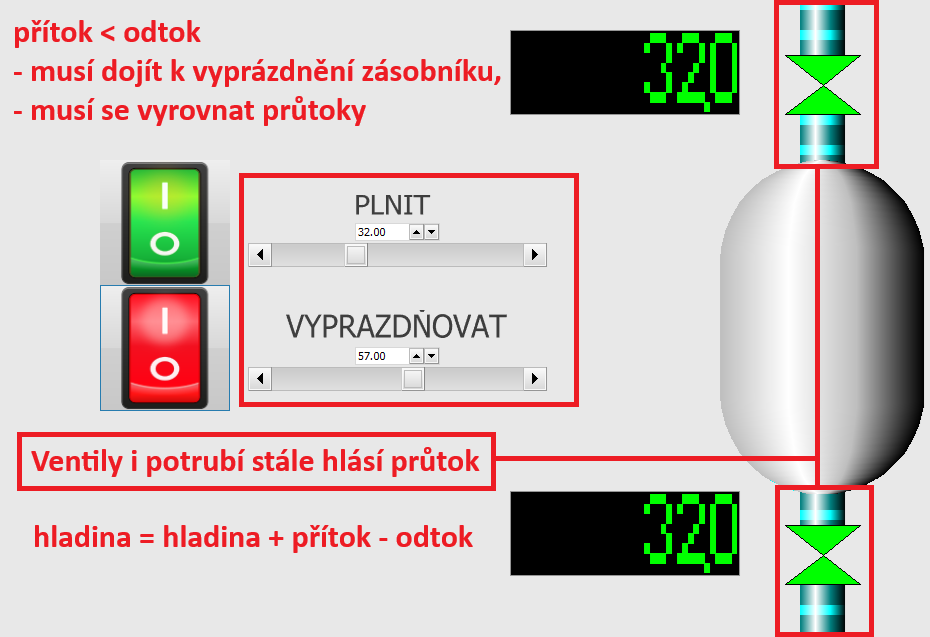
\includegraphics[width=0.85\textwidth]{fig/program_ukol_c.png}
		\end{center}
		
	\end{frame}
	
% =====================================================================================================================
	\begin{frame}
    \frametitle{Aplikace - neviditelné přístroje}
		
		\begin{minipage}[t][\textheight][t]{0.5\textwidth}
		\small
		\textbf{Grafický editor:}
		
			\begin{center}
				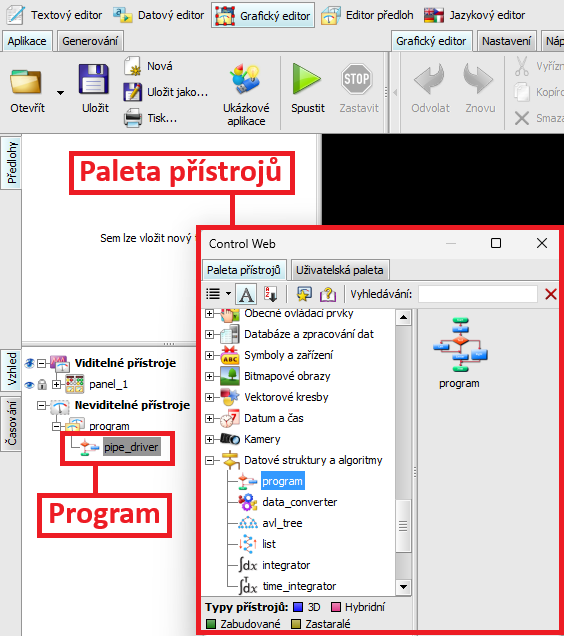
\includegraphics[width=1\textwidth]{fig/neviditelne_pristroje.png}
			\end{center}

		\end{minipage}
		\begin{minipage}[t][\textheight][t]{0.45\textwidth}
		
		\begin{itemize}
			\item Lze je využít pro například pro běh hlavní smyčky,
			\item stejně řešený datový inspektor,
			\item podobné procedury, jako například \textbf{OnActivate()}
		\end{itemize}

		\end{minipage}
		
	\end{frame}
	
% =====================================================================================================================
	\begin{frame}
    \frametitle{Aplikace - ovlivnění animace potrubí}
		
		\begin{center}
			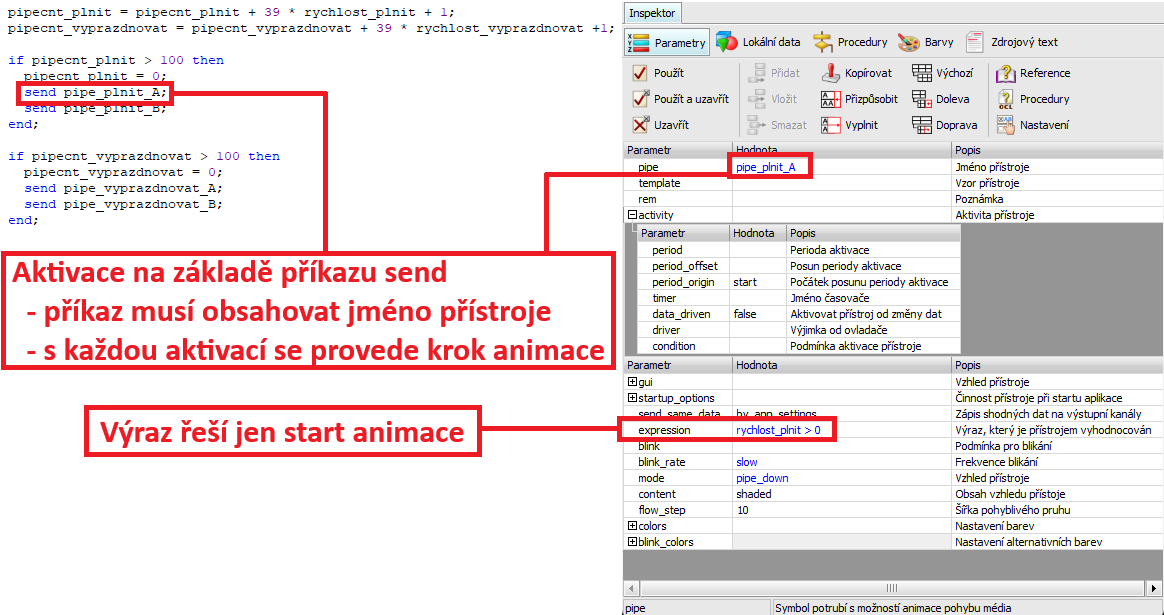
\includegraphics[width=1.00\textwidth]{fig/animace_potrubi.png}
		\end{center}
		
	\end{frame}